% How to use writeLaTeX: 
%
% You edit the source code here on the left, and the preview on the
% right shows you the result within a few seconds.
%
% Bookmark this page and share the URL with your co-authors. They can
% edit at the same time!
%
% You can upload figures, bibliographies, custom classes and
% styles using the files menu.
%
% If you're new to LaTeX, the wikibook is a great place to start:
% http://en.wikibooks.org/wiki/LaTeX
%
\documentclass{tufte-handout}

%\geometry{showframe}% for debugging purposes -- displays the margins

\usepackage{amsmath}
\usepackage{siunitx}

% Set up the images/graphics package
\usepackage{graphicx}
\setkeys{Gin}{width=\linewidth,totalheight=\textheight,keepaspectratio}
\graphicspath{{graphics/}}

\title{Fundamentos de Astrofísica\thanks{Inspired by Edward~R. Tufte!}}
\author[Alberto Garcia-Garcia]{Alberto Garcia-Garcia}
\date{\today}  % if the \date{} command is left out, the current date will be used

% The following package makes prettier tables.  We're all about the bling!
\usepackage{booktabs}

% The units package provides nice, non-stacked fractions and better spacing
% for units.
\usepackage{units}

\usepackage[americanvoltage]{circuitikz}
\usepackage{tikz}
\usetikzlibrary{arrows,shapes,positioning}
\usetikzlibrary{decorations.markings}

% The fancyvrb package lets us customize the formatting of verbatim
% environments.  We use a slightly smaller font.
\usepackage{fancyvrb}
\fvset{fontsize=\normalsize}

% Small sections of multiple columns
\usepackage{multicol}

% Provides paragraphs of dummy text
\usepackage{lipsum}

\usepackage[spanish]{babel}
\usepackage[utf8]{inputenc}

% These commands are used to pretty-print LaTeX commands
\newcommand{\doccmd}[1]{\texttt{\textbackslash#1}}% command name -- adds backslash automatically
\newcommand{\docopt}[1]{\ensuremath{\langle}\textrm{\textit{#1}}\ensuremath{\rangle}}% optional command argument
\newcommand{\docarg}[1]{\textrm{\textit{#1}}}% (required) command argument
\newenvironment{docspec}{\begin{quote}\noindent}{\end{quote}}% command specification environment
\newcommand{\docenv}[1]{\textsf{#1}}% environment name
\newcommand{\docpkg}[1]{\texttt{#1}}% package name
\newcommand{\doccls}[1]{\texttt{#1}}% document class name
\newcommand{\docclsopt}[1]{\texttt{#1}}% document class option name

\begin{document}

\maketitle% this prints the handout title, author, and date

\begin{abstract}
%
\end{abstract}

\tableofcontents

\clearpage

\section{Constantes}

$1 [\si{\angstrom}] = 0.1 ~[nm]$\\
$\sigma = 1.380 \cdot 10^{-23} [J \cdot K^{-1}]$\\
$\sigma_b = 8.617 \cdot 10^{-5} [eV \cdot K^{-1}]$\\
$\sigma = 1.380 \cdot 10^{-16} [erg \cdot K^{-1}]$\\ 

\clearpage

\section{Astronomía de Posición e Instrumentación Astronómica}

\clearpage

\section{Astrofisica Estelar}

\subsection{Luminosidad y Brillo}

La luminosidad $L~[erg \cdot s^{-1}]$ es la energía total emitida por unidad de tiempo mientras que el brillo $l~[erg \cdot s^{-1} \cdot m^{-2}]$ es la energía recibida por área y unidad de tiempo (es decir, el flujo de energía).

\marginnote{Problema 1. La constante solar es la cantidad de energía recibida en la parte externa de la atmósfera terrestre en forma de radiación solar, por unidad de tiempo y de superficie, y medida en un plano perpendicular a los rayos del Sol. El valor es de $1365~[W/m^2]$. Estima a qué distancia debemos colocar una bombilla de $100~[W]$ para que su flujo sea igual a la constante solar.\\

\begin{align}
  r = \sqrt{\frac{L}{4\pi l}} = \sqrt{\frac{100}{4\pi 1365}} = 0.076 [m]
\end{align}
}

Ambas magnitudes se relacionan de la siguiente forma: imaginemos una estrella de luminosidad $L$ rodeada por una esfera de radio $r$. Asumiendo que la luz no es absorbida durante su viaje hacia la esfera, el flujo $l$ medido a una distancia $r$ es inversamente proporcional al cuadrado de la distancia (\emph{inverse square law of light}):

\begin{align}
  l = \frac{L}{4\pi r^2}
\end{align}

\subsection{Escala de Magnitudes Estelares}

Utilizando la \emph{inverse square law}, podemos asignar una magnitud absoluta $M$ a cada estrella, la cual se define como la magnitud aparente $m$ de una estrella si se encontrara a $10 [pc]$ de distancia.

\marginnote{
Una diferencia de 5 magnitudes aparentes supone que la estrella de menor magnitud es 100 veces más brillante que la estrella de mayor magnitud, por lo que podemos expresar el ratio de sus flujos como \\\ \\

$\frac{l_0}{l} = 100^{(m_1 - m_2)/5}$\\\ \\

por lo que tomando logaritmos\\\ \\

$m_1 - m_2 = -2.5\log_{10}\frac{l}{l_0}$
}

\begin{align}
  m = -2.5 \log{\frac{l}{l_0}}
\end{align}

\begin{align}
  M = -2.5 \log{\frac{L}{L_0}}
\end{align}

Podemos de esta forma establecer una conexión entre la magnitud aparente, la magnitud absoluta y la distancia de una estrella:

\begin{align}
  100^{(m - M)/5} = \frac{l_{10}}{l} = (\frac{d}{10 [pc]})^2
\end{align}

Podemos por lo tanto determinar la distancia como

\begin{align}
  d = 10^{(m - M + 5)/5} [pc]
\end{align}

\marginnote{Tomando logaritmos podemos establecer el \emph{distance modulus}, es decir, la cantidad $m - M$:\\\ \\

$m - M = 5 \log_{10}(d) - 5 = 5 \log_{10}\frac{d}{10}$
}

De estas ecuaciones se desprende que para dos estrellas a la misma distancia, el ratio de su brillo es igual al ratio de sus luminosidades. Por lo tanto, tomando el Sol como una de esas estellas podemos obtener la relación entre la magnitud absoluta de una estrella y su luminosidad, así como entre su magnitud relativa y su brillo:

\begin{align}
  M = M_{\odot} - 2.5 \log_{10}\frac{L}{L_{\odot}}
\end{align}

\begin{align}
  m = M_{\odot} - 2.5 \log_{10}\frac{l}{l_{10, \odot}}
\end{align}

\subsection{Temperaturas Estelares}

Todos los objetos con temperatura por encima del cero absoluto emiten luz de todas las longitudes de onda con diferentes niveles de eficiencia. Un emisor ideal es aquél que absorbe toda la luz incidente y radia toda esta energía con un espectro denominado espectro de cuerpo negro. Dado que un emisor ideal no refleja luz se le conoce como cuerpo negro (\emph{blackbody}) y la radiación que emite se conoce como radiación de cuerpo negro. Las estrellas son cuerpos negros (por lo menos de forma aproximada).

\paragraph{Ley de Wien}

Un cuerpo negro de temperatura $T$ emite un espectro continua con cierta energía en cada longitud de onda de manera que existe un pico máximo de energía en la longitud de onda $\lambda_{max}$ . La relación entre esta longitud de onda máxima y la temperatura fue descubierta por Wien:

\begin{align}
  \lambda_{max} T = 0.290 [cm \cdot K]
\end{align}

\begin{align}
  \lambda_{max} T = (5000~[\si{\angstrom}])(5800~[K])
\end{align}

\marginnote{
  
\emph{Problema 2.} Expresa la temperatura ambiente (300 $K$) en $[eV]$ y calcula a qué temperatura corresponde una energía de 13.6 $[ev]$.\\\ \\

La temperatura y la energía se relacionan mediante la constante de Boltzmann $E = \sigma T$.\\\ \\

Una temperatura de $300 [K]$ corresponde a una energía $ E = \sigma T = 8.617 \cdot 10^{-5} \cdot 300 = 0.0259 [eV]$.\\\ \\

Por otro lado, una energía de $13.6 [eV]$ corresponde a una temperatura $T = E / \sigma = 13.6 / 8.617 \cdot 10^{-5} = 1.58 \cdot 10^{15} [K]$.\\

\rule{\linewidth}{0.4pt}
}

\paragraph{Ley de Boltzmann}

A medida que la temperatura de un cuerpo negro aumenta, también lo hace su energía emitida por segundo en todas las longitudes de onda. Este fenómeno, descubierto por el físico austríaco Josef Stefan Boltzmann se expresa en función del área de dicho cuerpo negro $A$ como:

\begin{align}
  L = A \sigma T^4 ~ [erg \cdot s^{-1}]
\end{align}

Combinando esta ecuación con el brillo, podemos determinar la temperatura efectiva $T_e$ de la superficie de una estrella:

\begin{align}
  l = \sigma T_e^4 [erg \cdot s^{-1} \cdot m^{-2}]
\end{align}

\marginnote{
La constante de Boltzmann relaciona temperatura absoluta y energía. Toma los siguientes valores:\\

$\sigma = 1.380 \cdot 10^{-23} [J \cdot K^{-1}]$\\
$\sigma = 8.617 \cdot 10^{-5} [eV \cdot K^{-1}]$\\
$\sigma = 1.380 \cdot 10^{-16} [erg \cdot K^{-1}]$\\ 
}

\subsection{Color y Temperatura}

\marginnote{
\emph{Problema 3.} Sirio es la estrella más brillante del cielo nocturno. Su paralaje es $p = 0.377 ["]$ y sus magnitudes aparentes son $U = -1.50$, $B = -1.46$ y $V = -1.46$.\\\ \\

La distancia a Sirio es por lo tanto $d = 1 / p = 1 / 0.377 = 2.65 [pc]$. Dicha cantidad equivale a $d = 2.65 \cdot 3.26 = 8.65 [ly]$ y $d = 2.65 \cdot 206265 = 5.44 \cdot 10^{15} [AU]$ o $d = 8.14 \cdot 10^{16} [cm]$.\\\ \\

Los índices de color de Sirio son $U-B = -0.04$ y $B-V = 0$. A partir de ellos podemos estimar una temperatura de $9900~[K]$ (tomando cualquier diagrama que relacione estos índices de color con la temperatura) o empleando la fórmula de Ballesteros:

$T = 4600 \left(\frac{1}{0.92(B-V) + 1.7} + \frac{1}{0.92(B-V) + 0.62}\right) \simeq 10000~[K] = 10000 \cdot \sigma_b = 0.86~[eV]$\\\ \\

La relación módulo-distancia $m - M = 5\log_{10}(d) - 5$ nos permite obtener las magnitudes absolutas cada una de las bandas en función de sus magnitudes relativas $U$, $B$, $V$ ya que $M = m + 2.88$ siendo $d = 2.65~[pc]$:\\

$M_U = -1.50 + 2.88 = 1.38$\\
$M_B = -1.46 + 2.88 = 1.42$\\
$M_V = -1.46 + 2.88 = 1.42$\\

}

Las magnitudes absolutas y aparentes medidas sobre todas las longitudes de onda de la luz emitida por una estrella se conocen como \emph{magnitudes bolométricas} $m_{bol}$ y $M_{bol}$. En la práctica, los detectores son sensibles a una cierta región de longitudes de onda. Así pues, el color de una estrella puede ser determinado con precisión empleando filtros que transmitan la luz de la estrella únicamente en ciertos rangos de longitudes de onda relativamente estrechos. Es el caso del sistema $UBV$ segundoún el cual la magnitud aparente de una estrella es determinada a partir de tres filtros:

\begin{itemize}
  \item U, la magnitud ultravioleta de la estrella (filtro centrado en $3650 [\si{\angstrom}]$ y con un ancho de banda de $680 [\si{\angstrom}]$).
  \item B, la magnitud azul de la estrella (filtro centrado en $4400 [\si{\angstrom}]$ y con un ancho de banda de $980 [\si{\angstrom}]$).
  \item V, la magnitud visual de la estrella (filtro centrado en $5500 [\si{\angstrom}]$ y con un ancho de banda de $890 [\si{\angstrom}]$).
\end{itemize}

Las magnitudes absolutas de color de la estrella $M_U$, $M_B$ y $M_V$ pueden determinarse si la distancia $d$ es conocida. Para ello, recurrimos a los índices de color $(U-B)$ y $(B-V)$:

\begin{align}
  U - B = M_U - M_B
\end{align}
\begin{align}
  B - V = M_B = M_V
\end{align}

\marginnote{
\emph{Problema 4.} Usando una temperatura efectiva para la estrella Vega de $9500~[K]$ y suponiendo que tenemos tres filtros de badna U,B,V con los siguientes valores de longitud de onda central y ancho de banda, determina en qué filtro se verá más brillante. $\lambda_U = 365~[nm]$, $\Delta\lambda_U = 68~[nm]$, $\lambda_B = 440~[nm]$, $\Delta\lambda_B = 98~[nm]$, $\lambda_V = 550~[nm]$, $\Delta\lambda_V = 89~[nm]$.\\\ \\

De acuerdo a la Ley de Wien, el espectro de Vega tiene un pico en la longitud de onda $\lambda_{max} = \frac{5000~[\si{\angstrom}] 5800~[K]}{9500~[K]} = 3052.63~[\si{\angstrom}] \approx 305~[nm]$, lo cual corresponde al espectro ultravioleta.
}

\subsection{Distancia a las Estrellas}

La distancia en pársecs a una estrella se puede determinar por su paralaje en segundos:

\begin{align}
  d = 1 / p [pc]
\end{align}

\clearpage

\section{El Sol}

\clearpage

\section{El Sistema Solar}

\subsection{El Cinturón de Asteroides}

Generalmente referido como el \emph{Main Belt} para diferenciarlo del \emph{Kuiper Belt}, se localiza entre las órbitas de Marte y Júpiter y cubre una distancia de alrededor de 2-3 $[UA]$ aunque en su mayoría consiste en espacio vacío, contiene trillones de rocas espaciales.

Cuatro objetos en él contienen más de la mitad de la masa total del cinturón (la cual se sitúa alrededor de un $4~\%$ de la masa de la Luna): Vesta, Pallas, Hygiea y el planeta enano Ceres.

La mayoría de los objetos del cinturón están compuestos de minerales y son ricos en hierro y níquel por lo que la teoría de mayor calado es que sean restos de la formación del Sistema Solar: una nube enorme de gas y partículas que poco a poco fueron acretando.

La sonda \emph{Dawn} fue enviada para investigarlo, la cual orbitó Vesta en 2011 descubriendo que se trata más bien de un protoplaneta más que de un trozo de roca. De la misma forma, se descubrió que Ceres tiene una capa de hielo-agua en 2015.

\subsection{Planetas Gigantes}

Más allá de Marte y del cinturón de asteroides se sitúan los dos planetas más grandes del Sistema Solar: los planetas gaseosos Júpiter y Saturno, principalmente compuestos por Helio e Hidrógeno (con mucha más cantidad del segundo que del primero). La principal teoría de su formación sostiene que se formaron al comienzo de la historia del Sistema Solar, lo cual les permitió acumular grandes cantidades de los dos gases más ligeros.

Júpiter está compuesto aproximadamente de $90~\%$ de hidrógeno y $10~\%$ de helio mientras que Saturno contiene un $96~\%$ de hidrógeno por únicamente un $3~\%$ de helio. Sin embargo, mientras que Júpiter es tremendamente masivo, Saturno tiene una densidad del $12\%$ respecto a la de la Tierra.

Júpiter posee el campo magnético más fuerte de todos los planetas del Sistema Solar y su radiación emitida es capaz de destruir sondas cercanas. La radiación emitida por Saturno es relativamente débil en comparación.

Aunque parezca contraintuitivo, ambos planetas poseen una superficie pese a ser gaseosos (localizada en el punto en el que la presión atmosférica es igual a la presión atmosférica en la superficie de la Tierra).

La sonda \emph{Galileo} en el año 2003 se estrelló contra la superficie de Júpiter registrando vientos de 700 $[km/h]$ y una temperatura de 151 grados centígrados justo antes de perder el contacto.

Creemos que ambos planetas poseen núcleos sólidos o al menos semi-sólidos. En cualquier caso, ambos núcleos internos están rodeados por una mezcla extraña de hidrógeno metálico líquido. Dadas las elevadas temperaturas y presiones cerca de ambos núcleos, se piensa que las moléculas de hidrógeno pueden soltar sus electrones convirtiéndose en metal líquido.

\subsection{Urano y Neptuno}

Tras Júpiter y Saturno se sitúan los dos planetas helados e invisibles al ojo humano en condiciones normales desde la Tierra: Urano y Neptuno. Son los dos planetas más desconocidos y la única sonda de la que tenemos datos es la Voyager 2 a finales de 1980.

Ambos planetas poseen tamaño (aproximadamente $50.000~[km]$), masa (alrededor de $14.5$ y $17$ veces la masa de la Tierra respectivamente) y composición similares.

Las atmósferas congeladas del exterior de ambos planetas contienen cantidades similares de los componentes principales hidrógeno, helio y metano (lo que les proporciona su famoso color azulado). Los mantos de ambos planetas están compuestos de agua, amoníaco y metano.

Urano no genera mucho calor interno por su cuenta por lo que se mantiene helado a una temperatura aproximada de $-220$ grados centígrados. En general, no tiene un clima cambiante dado que su eje de rotación hace que un polo esté constantemente (con un período de 42 años) hacia el sol.

Neptuno por su parte posee el clima más extremo, con vientos de hasta $2.100~[km/h]$ y tormentas de meses e incluso años. Su temperatura media es similar a la de Urano aunque su núcleo sí que emite una gran cantidad de calor.

\subsection{La Nube de Oort}

Contiene entre billones y hasta dos trillones de objetos helados principalmente compuestos de amoníaco, agua y metano. Se estima que tiene una anchura de un año luz y comienza a partir de $2000~[UA]$ de la Tierra.

\clearpage

\section{Sistemas Planetarios}

\clearpage

\section{Medio Interestelar}

\subsection{Polvo Cósmico}

\paragraph{Detección de Polvo}

Las nubes de polvo interestelar están demasiado frías como para irradiar energía en el espectro visible pero sí brillan con intensidad en el infrarrojo. Los pequeños granos de polvo absorben luz visible y radiación ultravioleta con eficiencia por lo que se calientan a temperaturas de $10-500~[K]$ radiando este calor en el infrarrojo.

\paragraph{Nebulosas de Reflexión}

Las \emph{Reflection nebula} ocurren cuando las nubes de polvo estelar se encuentran tan cerca de estrellas luminosas y hacen \emph{scatter} de suficiente luz como para que sean visibles. Lo que vemos, es la luz de la estrella reflejada en los granos de polvo estelar. Frecuentemente, parecen más azuladas que la luz real de la estrella que las ilumina ya que esas pequeñas partículas reflejan la luz azul con mayor eficiencia que la roja.

\paragraph{Nebulosas de Emisión}

TODO

\paragraph{Extinción Interestelar}

Los pequeños granos de polvo interestelar absorben parte de la luz de las estrellas que interceptan. Pero al menos la mitad de dicha luz es dispersada en lugar de absorberla. Como ni la luz absorbida ni la reflejada nos llega directamente, las estrellas parecen más tenues. El efecto combinado de estos dos procesos se denomina extinción.

Cabe destacar que el polvo no interactúa con todos los colores de la luz de la misma forma. La mayor parte de la luz azul, violeta y verde es dispersada y no nos alcanza. Mientras que otras luces con mayor longitud de onda como naranjas y rojos penetran en el polvo y sí que nos llegan a nosotros. Por este fenómeno, las estrellas parecen más rojas aunque sus líneas espectrales indiquen lo contrario.

\begin{figure}
  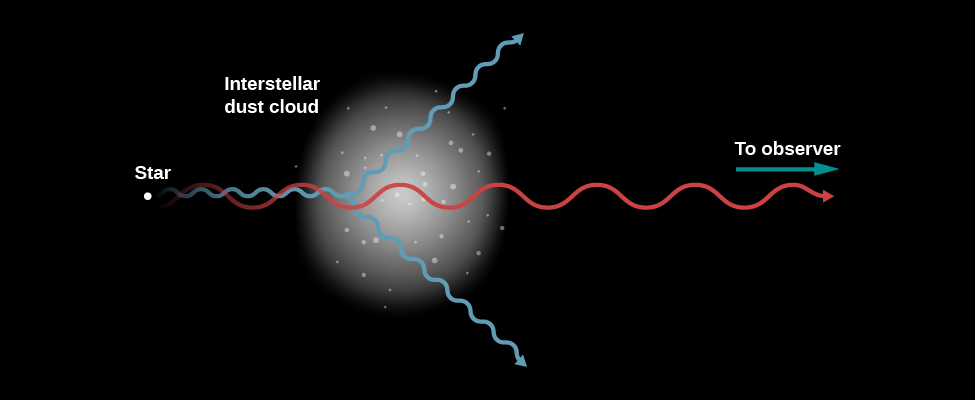
\includegraphics[width=\linewidth]{img/scatter}
  \caption{Dispersión o \emph{scattering} de la luz producida por polvo estelar.}
\end{figure}

\paragraph{Granos Interestelares}

La absorción y por lo tanto la extinción interestelar no puede provenir del gas. Tomando por ejemplo la Tierra, incluso con la altísima densidad de gas que posee nuestra atmósfera comparada con el medio interestelar, el gas sigue siendo prácticamente invisible por lo que la cantidad de gas interestelar debería mucho mayor de la existente para producir la absorción. En definitiva, el causante de este fenómeno debe ser un conjunto de partículas muy dispersas y de diversa composición: principalmente hidrógeno, helio, oxígeno, carbono y nitrógeno.

Estas partículas en su mayoría pueden caracterizarse como \emph{sootlike} (ricas en carbón) o \emph{sandlike} (conteniendo silicio y oxígeno). El modelo más extendido de estos granos supone un núcleo rocoso rico en carbono o silicatos rodeado de mantos helados de agua, metano o amoníaco.

Estos granos deben ser ligeramente inferiores en tamaño a la longitud de onda de la luz visible en torno a $10-100~[nm]$(si fueran más pequeños, la luz no sería bostruida; si fueran mayores, no se produciría el enrojecimiento).

\subsection{Rayos Cósmicos}

Además de gas y polvo, existe un tercer tipo de partículas que se encuentra en el espacio interestelar: rayos cósmicos. Se trata de partículas de composición similar al gas interestelar pero que viajan a altas velocidades (típicamente al $90~\%$ de la velocidad de la luz). La mayoría de ellos son núcleos de hidrógeno sin su electrón.

Dado que se tratan de partículas con carga, su trayectoria se ve afectada por campos magnéticos; eso provoca que sea casi imposible determinar su origen. Se supone que se originan en el interior de la galaxia (puesto que los campos magnéticos en el espacio interestelar son suficientemente fuertes como para prevenir su escape); el mejor candidato para su origen es la explosión de una supernova.

\subsection{El Ciclo Vital del Material Cósmico}

\paragraph{Flujo de Gas Interestelar}

La masa total del medio interestelar depende del tira y afloja entre aquella que se gana (por gravedad) del espacio intergaláctico, la conversión de parte de la misma en estrellas, y la pérdida provocada por masa devuelta de nuevo al espacio intergaláctico por la explosión de supernovas. Este proceso se conoce como el ciclo de \emph{baryon}.

\paragraph{Ciclo del Polvo y Elementos Pesados}

Aunque la mayor parte de la masa del medio interestelar se debe a material acretado del espacio intergaláctico, eso no explica los elementos más pesados que el hidrógeno y el helio ni tampoco el polvo estelar.

Los elementos pesados son formados en el interior de las estrellas de la Vía Láctea y son devueltos al medio interestelar al final de sus vidas.

Un proceso similar ocurre para los granos de polvo cósmico, que se forman al condensarse en regiones donde el gas es denso y frío (por ejemplo en los vientos de estrellas luminosas frías) o al enfriarse los gases eyectados por una supernova. Los "escudos" de hielo de estos granos serán evaporados por estrellas calientes e incorporados a su masa, creando de nuevo un ciclo.

\subsection{Material Interestelar alrededor del Sol}

\begin{figure}
  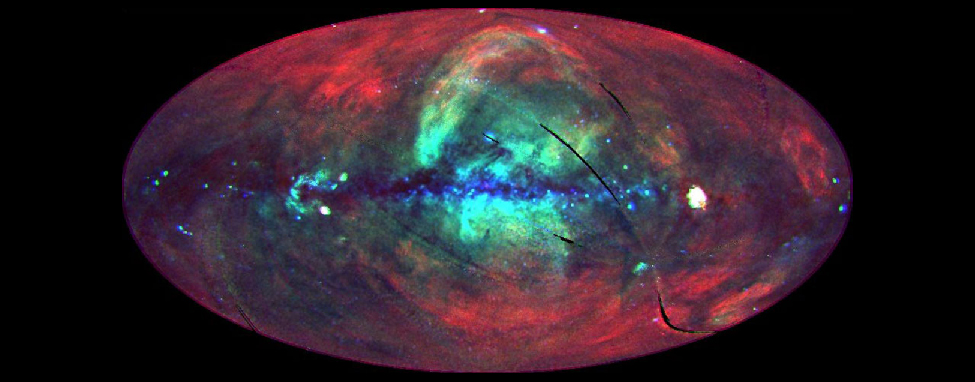
\includegraphics[width=\linewidth]{img/xray}
  \caption{Cielo en rayos X capturado por el satélite ROSAT; en rojo las regiones menos energéticas y en azul las más.}
\end{figure}

Los telescopios de rayos X han mostrado que la Galaxia está llena de burbujas de gases calientes emisores de rayos X. También han observado un fondo difuso de rayos X en todo el cielo desde nuestra perspectiva. Aunque una parte de ellos proviene de la interacción del viento solar con el medio interestelar, gran parte proviene de fuera del sistema solar. La explicación lógica a que haya gas caliente emisor de rayos X alrededor nuestro es que el Sol esté localizado en una de dichas burbujas conocida como la \emph{Local Hot Bubble}, mucho menos densa que el la densidad media interestelar (1 átomo por $cm^3$).

\section{Medio Interestelar: Review Questions}

\paragraph{Identify several dark nebulae in photographs in this chapter. Give the figure numbers of the photographs,
and specify where the dark nebulae are to be found on them.}

\paragraph{\textbf{Why do nebulae near hot stars look red? Why do dust clouds near stars usually look blue?}}

El gas interestelar cerca de las estrellas calientes es a su vez calentado a temperaturas de hasta $10000~[K]$, a su vez, la radiación ultravioleta de la estrella ioniza las nubes de gas. Como el hidrógeno es el principal componente de las mismas, se convierten en regiones $HII$ que están continuamente capturando electrones libres y perdiéndolos por ionización. Durante este proceso, emiten luz por fluorescencia y como generalmente el hidrógeno es su principal constituyente, la línea más fuerte en el espectro visible es la roja del hidrógeno. Este fenómeno se conoce como nebulosas de emisión.

Por otro lado, las nubes de polvo reflejan y dispersan la luz emitida por las estrellas cercanas. Al impactar contra el polvo estelar, la luz de longitud de onda azul se refleja de forma más eficiente que la roja por lo que parecen emitir un brillo azul. Se conocen como nebulosas de reflexión.

\paragraph{\textbf{Describe the characteristics of the various kinds of interstellar gas (HII regions, neutral hydrogen clouds,
ultra-hot gas clouds, and molecular clouds).}}

Las regiones $HII$ se tratan de gases (principalmente compuestos de hidrógeno) cerca de estrellas calientes que son ionizados por la radiación ultravioleta de dichas estrellas. Emiten luz roja por fluorescencia y se conocen como nebulosas de emisión.

Las nubes de hidrógeno neutral son las más comunes ya que las estrellas calientes necesarias para las regiones $HII$ son escasas y solamente una pequeña fracción del gas interestelar se encuentra lo suficientemente cerca para que se produzcan. A temperaturas típicas del medio interestelar ni absorben ni emiten luz en el espectro visible. Son detectables por líneas de absorción estrechas en determinadas partes fuera del espectro visible (principalmente a causa de calcio y sodio).

Las nubes de gas ultra-calientes se encuentran a temperaturas de un millón de grados centígrados o más (descubierto debido a que contienen átomos de oxígeno ionizados cinco veces). Se teoriza que este tipo de nubes son producidas por la explosión de una supernova.

Las nubes moleculares son regiones en las que la interacción gravitatoria ha atraído gas interestelar los suficiente para formar estructuras masivas de moléculas procedentes de la acumulación de polvo estelar en dicha región por la atracción gravitatoria. Estas nubes masivas producen una nube oscura que bloquean la luz ultravioleta y visible de las estrellas.

\paragraph{\textbf{Prepare a table listing the different ways in which dust and gas can be detected in interstellar space.}}

(1) Bloqueando directamente la luz visible, (2) reflejando/absorbiendo la luz de una estrella cercana, (3) emisiones de infrarrojos.

\paragraph{\textbf{Describe how the 21-cm line of hydrogen is formed. Why is this line such an important tool for
understanding the interstellar medium?}}

Un átomo de hidrógeno neutro excitado (en nuestro caso por la colisión con otros átomos de hidrógeno o con electrones libres), puede acabar perdiendo ese exceso de energía de excitación de nuevo o bien colisionando con otra partícula o bien emitiendo radiación con una longitud de onda de $21~[cm]$. Este proceso es lento (de media se produce una espera de $10~[Myr]$); aunque, dada la inmensa cantidad de átomos de hidrógeno en una nube neutra se produce con bastante asiduidad. La creación de equipo con sensibilidad suficiente para dicha longitud de onda ha permitido la detección de nubes de hidrógeno neutro en el medio interestelar.

\paragraph{\textbf{Describe the properties of the dust grains found in the space between stars.}}

TODO

\paragraph{\textbf{Why is it difficult to determine where cosmic rays come from?}}

Las partículas de un rayo cósmico están cargadas por lo que se ven afectadas por los diversos campos magnéticos presentes en el medio interestelar que desvían su trayectoria. Además, por la propia acción del campo magnético terrestre suelen sufrir varios cambios en la trayectoria antes de alcanzar la atmósfera en la cual los podemos detectar.

\paragraph{\textbf{What causes reddening of starlight? Explain how the reddish color of the Sun’s disk at sunset is caused by
the same process.}}

Los granos de polvo interestelar producen dispersión de las longitudes de onda azules mientras que las rojas apenas se ven afectadas; esto provoca que cuando dicha radiación nos llega a nosotros como observadores capturamos más luz roja que la que realmente emiten las estrellas. En realidad, el proceso es más bien un \emph{deblueing} más que \emph{reddening}. Este mismo proceso pero producido por las partículas presentes en nuestra atmósfera causa que el cielo tenga un color azulado (\emph{scattering}) mientras que el disco del sol parezca más rojo en la puesta (dado también el ángulo de incidencia de los rayos).

\paragraph{\textbf{Why do molecules, including $H_2$ and more complex organic molecules, only form inside dark clouds? Why
don’t they fill all interstellar space?}}

Únicamente se forman en el interior de nubes oscuras debido a que esa acumulación de materia bloquea la radiación ultravioleta de las estrellas cercanas, impidiendo así el proceso de ionización que a su vez haría imposible la formación de moléculas mayores y complejas. Esto no ocurre en todo el espacio interestelar puesto que los granos de polvo son una mínima parte de su composición y estas nubes masivas únicamente se forman en regiones muy concretas debido a atracción gravitatoria significativa.

\paragraph{\textbf{Why can't we use visible light telescopes to study molecular clouds where stars and planets form? Why do
infrared or radio telescopes work better?}}

Las nubes moleculares emiten radiación en una longitud de onda mayor que la de la luz visible. Es por ello que los telescopios infrrarojos ofrecen una mejor solución para captar dicha radiación.

\paragraph{The mass of the interstellar medium is determined by a balance between sources (which add mass) and
sinks (which remove it). Make a table listing the major sources and sinks, and briefly explain each one.}

\paragraph{Where does interstellar dust come from? How does it form?}

\section{Medio Interestelar: Thought Questions}

\clearpage

\section{Galaxias}

\clearpage

\section{Cosmología Física}

\clearpage

% \subsection{Sidenotes}\label{sec:sidenotes}
% One of the most prominent and distinctive features of this style is the
% extensive use of sidenotes.  There is a wide margin to provide ample room
% for sidenotes and small figures.  Any \Verb|\footnote|s will automatically
% be converted to sidenotes.\footnote{This is a sidenote that was entered
% using the \texttt{\textbackslash footnote} command.}  If you'd like to place ancillary
% information in the margin without the sidenote mark (the superscript
% number), you can use the \Verb|\marginnote| command.\marginnote{This is a
% margin note.  Notice that there isn't a number preceding the note, and
% there is no number in the main text where this note was written.}

% The specification of the \Verb|\sidenote| command is:
% \begin{docspec}
%   \doccmd{sidenote[\docopt{number}][\docopt{offset}]\{\docarg{Sidenote text.}\}}
% \end{docspec}

% Both the \docopt{number} and \docopt{offset} arguments are optional.  If you
% provide a \docopt{number} argument, then that number will be used as the
% sidenote number.  It will change of the number of the current sidenote only and
% will not affect the numbering sequence of subsequent sidenotes.

% Sometimes a sidenote may run over the top of other text or graphics in the
% margin space.  If this happens, you can adjust the vertical position of the
% sidenote by providing a dimension in the \docopt{offset} argument.  Some
% examples of valid dimensions are:
% \begin{docspec}
%   \ttfamily 1.0in \qquad 2.54cm \qquad 254mm \qquad 6\Verb|\baselineskip|
% \end{docspec}
% If the dimension is positive it will push the sidenote down the page; if the
% dimension is negative, it will move the sidenote up the page.

% While both the \docopt{number} and \docopt{offset} arguments are optional, they
% must be provided in order.  To adjust the vertical position of the sidenote
% while leaving the sidenote number alone, use the following syntax:
% \begin{docspec}
%   \doccmd{sidenote[][\docopt{offset}]\{\docarg{Sidenote text.}\}}
% \end{docspec}
% The empty brackets tell the \Verb|\sidenote| command to use the default
% sidenote number.

% If you \emph{only} want to change the sidenote number, however, you may
% completely omit the \docopt{offset} argument:
% \begin{docspec}
%   \doccmd{sidenote[\docopt{number}]\{\docarg{Sidenote text.}\}}
% \end{docspec}

% The \Verb|\marginnote| command has a similar \docarg{offset} argument:
% \begin{docspec}
%   \doccmd{marginnote[\docopt{offset}]\{\docarg{Margin note text.}\}}
% \end{docspec}

% \subsection{References}
% References are placed alongside their citations as sidenotes,
% as well.  This can be accomplished using the normal \Verb|\cite|
% command.\sidenote{The first paragraph of this document includes a citation.}

% The complete list of references may also be printed automatically by using
% the \Verb|\bibliography| command.  (See the end of this document for an
% example.)  If you do not want to print a bibliography at the end of your
% document, use the \Verb|\nobibliography| command in its place.  

% To enter multiple citations at one location,\cite{Tufte2006,Tufte1990} you can
% provide a list of keys separated by commas and the same optional vertical
% offset argument: \Verb|\cite{Tufte2006,Tufte1990}|.  
% \begin{docspec}
%   \doccmd{cite[\docopt{offset}]\{\docarg{bibkey1,bibkey2,\ldots}\}}
% \end{docspec}

% \section{Figures and Tables}\label{sec:figures-and-tables}
% Images and graphics play an integral role in Tufte's work.
% In addition to the standard \docenv{figure} and \docenv{tabular} environments,
% this style provides special figure and table environments for full-width
% floats.

% Full page--width figures and tables may be placed in \docenv{figure*} or
% \docenv{table*} environments.  To place figures or tables in the margin,
% use the \docenv{marginfigure} or \docenv{margintable} environments as follows
% (see figure~\ref{fig:marginfig}):

% \begin{marginfigure}%
%   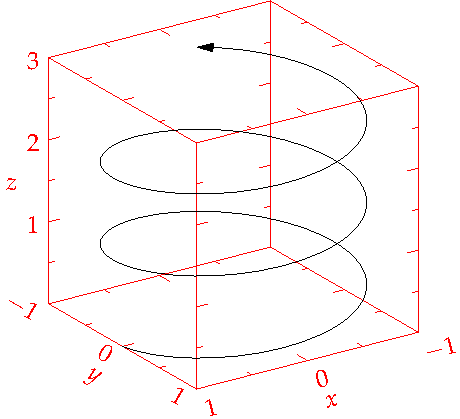
\includegraphics[width=\linewidth]{helix}
%   \caption{This is a margin figure.  The helix is defined by 
%     $x = \cos(2\pi z)$, $y = \sin(2\pi z)$, and $z = [0, 2.7]$.  The figure was
%     drawn using Asymptote (\url{http://asymptote.sf.net/}).}
%   \label{fig:marginfig}
% \end{marginfigure}
% \begin{Verbatim}
% \begin{marginfigure}
%   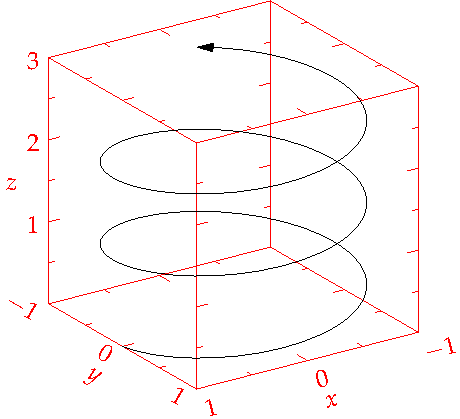
\includegraphics{helix}
%   \caption{This is a margin figure.}
% \end{marginfigure}
% \end{Verbatim}

% The \docenv{marginfigure} and \docenv{margintable} environments accept an optional parameter \docopt{offset} that adjusts the vertical position of the figure or table.  See the ``\nameref{sec:sidenotes}'' section above for examples.  The specifications are:
% \begin{docspec}
%   \doccmd{begin\{marginfigure\}[\docopt{offset}]}\\
%   \qquad\ldots\\
%   \doccmd{end\{marginfigure\}}\\
%   \mbox{}\\
%   \doccmd{begin\{margintable\}[\docopt{offset}]}\\
%   \qquad\ldots\\
%   \doccmd{end\{margintable\}}\\
% \end{docspec}

% Figure~\ref{fig:fullfig} is an example of the \Verb|figure*|
% environment and figure~\ref{fig:textfig} is an example of the normal
% \Verb|figure| environment.

% \begin{figure*}[h]
%   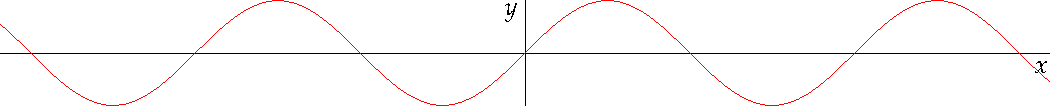
\includegraphics[width=\linewidth]{sine.pdf}%
%   \caption{This graph shows $y = \sin x$ from about $x = [-10, 10]$.
%   \emph{Notice that this figure takes up the full page width.}}%
%   \label{fig:fullfig}%
% \end{figure*}

% \begin{figure}
%   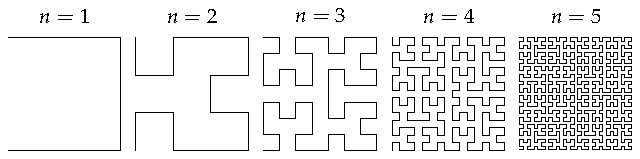
\includegraphics{hilbertcurves.pdf}
% %  \checkparity This is an \pageparity\ page.%
%   \caption{Hilbert curves of various degrees $n$.
%   \emph{Notice that this figure only takes up the main textblock width.}}
%   \label{fig:textfig}
%   %\zsavepos{pos:textfig}
%   \setfloatalignment{b}
% \end{figure}

% Table~\ref{tab:normaltab} shows table created with the \docpkg{booktabs}
% package.  Notice the lack of vertical rules---they serve only to clutter
% the table's data.

% \begin{table}[ht]
%   \centering
%   \fontfamily{ppl}\selectfont
%   \begin{tabular}{ll}
%     \toprule
%     Margin & Length \\
%     \midrule
%     Paper width & \unit[8\nicefrac{1}{2}]{inches} \\
%     Paper height & \unit[11]{inches} \\
%     Textblock width & \unit[6\nicefrac{1}{2}]{inches} \\
%     Textblock/sidenote gutter & \unit[\nicefrac{3}{8}]{inches} \\
%     Sidenote width & \unit[2]{inches} \\
%     \bottomrule
%   \end{tabular}
%   \caption{Here are the dimensions of the various margins used in the Tufte-handout class.}
%   \label{tab:normaltab}
%   %\zsavepos{pos:normaltab}
% \end{table}

% \section{Full-width text blocks}

% In addition to the new float types, there is a \docenv{fullwidth}
% environment that stretches across the main text block and the sidenotes
% area.

% \begin{Verbatim}
% \begin{fullwidth}
% Lorem ipsum dolor sit amet...
% \end{fullwidth}
% \end{Verbatim}

% \begin{fullwidth}
% \small\itshape\lipsum[1]
% \end{fullwidth}

% \section{Typography}\label{sec:typography}

% \subsection{Typefaces}\label{sec:typefaces}
% If the Palatino, \textsf{Helvetica}, and \texttt{Bera Mono} typefaces are installed, this style
% will use them automatically.  Otherwise, we'll fall back on the Computer Modern
% typefaces.

% \subsection{Letterspacing}\label{sec:letterspacing}
% This document class includes two new commands and some improvements on
% existing commands for letterspacing.

% When setting strings of \allcaps{ALL CAPS} or \smallcaps{small caps}, the
% letter\-spacing---that is, the spacing between the letters---should be
% increased slightly.\cite{Bringhurst2005}  The \Verb|\allcaps| command has proper letterspacing for
% strings of \allcaps{FULL CAPITAL LETTERS}, and the \Verb|\smallcaps| command
% has letterspacing for \smallcaps{small capital letters}.  These commands
% will also automatically convert the case of the text to upper- or
% lowercase, respectively.

% The \Verb|\textsc| command has also been redefined to include
% letterspacing.  The case of the \Verb|\textsc| argument is left as is,
% however.  This allows one to use both uppercase and lowercase letters:
% \textsc{The Initial Letters Of The Words In This Sentence Are Capitalized.}



% \section{Installation}\label{sec:installation}
% To install the Tufte-\LaTeX\ classes, simply drop the
% following files into the same directory as your \texttt{.tex}
% file:
% \begin{quote}
%   \ttfamily
%   tufte-common.def\\
%   tufte-handout.cls\\
%   tufte-book.cls
% \end{quote}

% % TODO add instructions for installing it globally



% \section{More Documentation}\label{sec:more-doc}
% For more documentation on the Tufte-\LaTeX{} document classes (including commands not
% mentioned in this handout), please see the sample book.

% \section{Support}\label{sec:support}

% The website for the Tufte-\LaTeX\ packages is located at
% \url{http://code.google.com/p/tufte-latex/}.  On our website, you'll find
% links to our \smallcaps{svn} repository, mailing lists, bug tracker, and documentation.

\bibliography{sample-handout}
\bibliographystyle{plainnat}



\end{document}